\documentclass[%
		%draft,
    %submission,
    %compressed,
    final,
    %
    %technote,
    %internal,
    %submitted,
    %inpress,
    reprint,
    %
    %titlepage,
    notitlepage,
    %anonymous,
    narroweqnarray,
    inline,
    twoside,
    invited
    ]{ieee}

\usepackage[utf8]{inputenc}
\usepackage[spanish]{babel}
\usepackage{graphicx}
\usepackage{verbatim}
\usepackage{moreverb}
\usepackage{amsmath}
\usepackage{amsfonts}
\usepackage{amssymb}
\usepackage{fancybox}
\usepackage{float}
\usepackage{fancyvrb}
\usepackage{subfigure}

\newcommand{\latexiie}{\LaTeX2{\Large$_\varepsilon$}}

%\usepackage{ieeetsp}    % if you want the "trans. sig. pro." style
%\usepackage{ieeetc}    % if you want the "trans. comp." style
%\usepackage{ieeeimtc}    % if you want the IMTC conference style

% Use the `endfloat' package to move figures and tables to the end
% of the paper. Useful for `submission' mode.
%\usepackage {endfloat}

% Use the `times' package to use Helvetica and Times-Roman fonts
% instead of the standard Computer Modern fonts. Useful for the 
% IEEE Computer Society transactions.
%\usepackage{times}
% (Note: If you have the commercial package `mathtime,' (from 
% y&y (http://www.yandy.com), it is much better, but the `times' 
% package works too). So, if you have it...
%\usepackage {mathtime}

% for any plug-in code... insert it here. For example, the CDC style...
%\usepackage{ieeecdc}

\begin{document}

%----------------------------------------------------------------------
% Title Information, Abstract and Keywords
%----------------------------------------------------------------------
\title[Redes de Hopfield]{%
       Redes de Hopfield}

% format author this way for journal articles.
% MAKE SURE THERE ARE NO SPACES BEFORE A \member OR \authorinfo
% COMMAND (this also means `don't break the line before these
% commands).
\author[Castiglione, Karpovsky, Sturla]{Gonzalo V. Castiglione, Alan E. Karpovsky, Martín Sturla\\\textit{Estudiantes 
       Instituto Tecnológico de Buenos Aires (ITBA)}\\
\textbf{12 de Mayo de 2012}
}


\journal{Cátedra\ \ Sist.\ de\ Inteligencia\ Artificial,\ ITBA\ }
\titletext{-\ 12, MAYO\ 2012}
\ieeecopyright{\copyright\ 2012 ITBA}
\lognumber{}
\pubitemident{}
\loginfo{12 de Mayo, 2012.}
\firstpage{1}

\confplacedate{Buenos Aires, Argentina, 12 de Mayo, 2012}

\maketitle               

\begin{abstract} 
El presente informe busca analizar la implementación de una Red de Hopfield con el fin de analizar su funcionalidad y comportamiento como memoria asociativa direccionable por el contenido.
\end{abstract}

\begin{keywords}
memoria asociativa direccionable por el contenido, hopfield, imágenes, memorización, ruido, atractores, estados espúreos
\end{keywords}

%----------------------------------------------------------------------
% SECTION I: Introduccion%----------------------------------------------------------------------
\section{Introducción}

\par Se analizó el comportamiento de una Red de hopfield como memoria asociativa direccionable por el contenido.\\
El trabajo consistió en la implementación una Red de Hopfield en el lenguaje \textit{Java}. Se tomó un conjunto de patrones a memorizar los cuales pueden visualizarse en la sección \textbf{\textit{Anexo A: Patrones}} y se realizaron numerosas pruebas con el fin de evaluar cuestiones como ser si los patrones son verdaderos atractores, cuál es la máxima cantidad de patrones que la red puede memorizar, qué sucede si se le da como entrada a la red un patrón con ruido, etc.\\
\par Si bien el algoritmo de hopfield es asincrónico, se decidió implementar una variante sincrónica del mismo para comprar los resultados obtenidos con cada uno.\\
\par En las siguientes secciones se desrrollará el modelado del problema como así también los resultados obtenidos y las conclusiones que se pueden extraer de ellos.


%----------------------------------------------------------------------
% SECTION II: Marco Teórico
%----------------------------------------------------------------------

\section{Desarrollo}

\subsection{Modelado del problema}

\par Algunas definiciones preliminares:\\
\begin{itemize}
\item \textbf{$\Psi$}: Conjunto de patrones a memorizar
\item \textbf{$N$}: Longitud de los patrones de entrada (ej. $N = 64$ si cada imagen es de $8x8$ pixels)
\item \textbf{$p$}: Cantidad de patrones distintos que contiene $\Psi$\\
\end{itemize}

\par Se representó a la Red de Hopfield en \textit{Java} como una clase abstracta debido a la distinción antes nombrada del algoritmo \textbf{sincrónico} versus el algoritmo \textbf{asincrónico} (nos permite hacer implementaciones concretas que extiendan de ella).\\
La clase contiene dos variables: un vector y una matriz que están definidos como sigue:\\

\begin{itemize}
\item \textbf{float[N][N] weights}: Matriz de pesos $W_{ij}$ correspondientes a los patrones que se desean memorizar.
\item \textbf{int[N] states;}: Vector con los estados de cada una de las $N$ neuronas.\\
\end{itemize}

\par Nótese que si bien el vector de estados es de tipo entero, los estados definidos para este problema son $1$ o $-1$ dado que las unidades que estamos utilizando son \textbf{bipolares}\\

\par Por otra parte se decidió representar a los patrones $\mu$ como vectores de enteros \textbf{\textit{int[] pattern}} los cuales contienen un $1$ en la posición $i$ en el caso de que el i-ésimo pixel del patrón sea negro o contienen un $-1$ en la posición $i$ en el caso de que el i-ésimo pixel del patrón sea blanco.\\
Todos los patrones de entrada fueron \textit{normalizados}, es decir que las imágenes cuyo mapa de color estaba en escala de grises fueron pasadas a imágenes blanco y negro; asimismo una de las imágenes que no contenía fondo (fondo transparende) fue modificada dejando intacta la imagen pero agregandole un fondo blanco.
	

\subsection{Inicialización de la red}

\par Se escribió un método \textit{storePatterns} inicializa la matriz de pesos sinápticos de la red neuronal utilizando la regla del producto externo de \textit{Hebb}. Nótese que la matriz de pesos, una vez inicializada, no cambia durante toda la ejecución del algoritmo.\\
Por cuestiones de eficiencia y dado que la matriz de pesos es simétrica con $W_{ij} = 0$, el algoritmo recorre sólo la diagonal superior de la misma y \textbf{espeja} los resultados.

\subsection{Función de activación}

\par La función de activación utizada es la función signo \textbf{f(x) = sgn(x)}.

\subsection{Actualización de estados}

\par Como ya se comentó, se implementaron dos variantes para la actualización de estados: el Modelo de Little y el Modelo de Hopfield los cuales se desarrollarán a continuación. En líneas generales ambos buscan iterar hasta la convergencia (el vector de estados de la red no cambia respecto del paso anterior). Ambas son equivalentes excepto por la distribución del intervalo de actualizaciones. El modelo de Hopfield da una secuencia aleatoria por lo cual hay baja probabilidad de que dos unidades elijan ser actualizadas en el mismo momento.\\
La primera es útil para simulaciones y la segunda es apropiada para unidades de hardware autónomas.\\
\par Es importante destacar que el método de iteración hasta la convergencia puede caer en \textbf{ciclos de longitud 2} por lo que es sumamente importante no sólo chequear que el vector de estados no haya cambiado respecto del paso anterior sino también hay que hacer esta verificación respecto de 2 pasos anteriores.

\subsubsection{Sincrónica (Modelo de Little)}

\par En cada paso se actualizan todas las neuronas de forma simultánea de acuerdo a la siguiente regla:\\

\begin{equation}
\label{updateRule}
S_i(n+1) = sgn\left(\sum_{j=1}^{N}{W_{ij}S_j(n)}\right)
\end{equation}

\subsubsection{Asincrónica (Modelo de Hopfield)}

\par En cada paso se actualiza una unidad por ves; la misma es seleccionada de forma completamente aleatoria y se utiliza la ecuación \ref{updateRule} para la actualización.

\subsection{Interfaz gráfica}

\section{Resultados}

\subsection{Verdaderos atractores}

\subsection{Estados espúreos}

\subsection{Patrones con ruido o incompletos}

\subsection{Patrones invertidos}

\subsection{Patrones desconocidos}

\subsection{Cantidad de patrones almacenables}

\par Como punto sumamente importante se obserbó que la \textbf{cantidad máxima de patrones posibles de almacenar} fue de XXXXXXXXXXXXXXXXX. Esto se puede explicar por YYYYYYYY.



\section{Conclusión}




%----------------------------------------------------------------------


\clearpage
\onecolumn

\section*{Anexo A: Patrones}

\begin{figure}[H]
\begin{center}
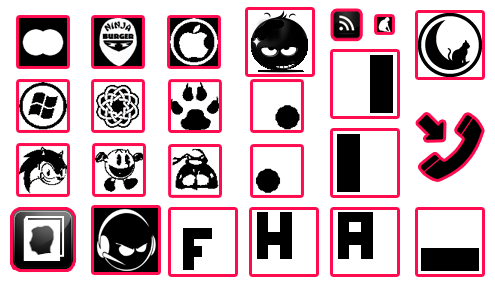
\includegraphics[scale=0.70]{./images/patterns.png}
\label{modelado}
\end{center}
\end{figure}

\begin{center}
\par Figura 1: Visualización de los 25 patrones con la que se inicializa a la red
\end{center}



%\VerbatimInput{./code/calculoAb.m}




\end{document}